\section{Introduction}\label{Introduction}

%%%%%%%%%%%%%%%%%%%%%%%%%%%%%%%%%%%%%%

\subsection{Motivation and Related Work}

Uncrewed aerial vehicles (UAVs), commonly known as drones, are expected to contribute to extraordinary economic growth and societal transformations. Thanks to their low cost and high mobility, UAVs will become of paramount importance for goods delivery, surveillance, search and rescue, and the monitoring of wildfire, crowds, and assets \cite{GerGarAza2022,wu20205g,UAVfire2022}. With rising urbanization pushing ground transportation to its limits, electrical vertical take-off and landing vehicles (eVTOLs) serving as air taxis or ambulances would take urban mobility to new heights, contributing to a faster, safer, and more interconnected transportation system. Autonomous levitating pods are no longer science fiction as projects and tests are underway, and they could redefine how we commute and, in turn, where we live and work \cite{SaeAlnAlo2020}. 
For these and other applications, UAVs will need to exchange an unprecedented amount of real-time data with the network, requiring ultra-reliable wireless connectivity. The latter must support safe UAV operations through low-latency control and mission-specific data payloads, persuading legislators to ease the current regulations on civilian pilotless flights and giving the green light to autonomous UAVs and the associated vertical markets \cite{FotQiaDin2019,ZenGuvZha2020,SaaBenMoz2020,NamChaKim17,CDHJGC20}.

Achieving fly-and-connect capabilities faces important hurdles. Traditional cellular base stations (BSs) are designed to optimize 2D connectivity on the ground. As a result, UAVs can only be reached by their upper antenna sidelobes, and their movement causes sharp signal fluctuations. In addition, UAVs flying above buildings receive and create line-of-sight (LoS) interfering signals from a plurality of BSs. This interference results in UAVs experiencing a degraded signal-to-interference-plus-noise ratio (SINR), which hinders the correct decoding of critical command and control messages \cite{GerGarGal2018,ZenLyuZha2019}. 
The mobile industry and academia have long joined forces to pursue \emph{3D connectivity}, i.e., also up in the air, by re-engineering the deployments originally built for the ground. Short-term solutions are being implemented to handle a few network-connected UAVs without compromising the performance of existing ground users, e.g., via time/frequency separation \cite{NguAmoWig2018,3GPP36777}. However, this approach becomes increasingly inefficient as the number of UAVs grows because it requires dedicated radio resources for each UAV. 
More advanced proposals for ubiquitous aerial connectivity rely on network densification \cite{GarGerLop2019,KanMezLoz2021,DanGarGer2020,CDALHJTWC22}, dedicated infrastructure for aerial services \cite{GerLopBen2022,KimKimRyu2022,MozLinHay2021}, or satellites complementing the ground network \cite{BenGerLop2022}. Nonetheless, these proposals may require costly hardware or signal processing upgrades and still face difficulties providing ubiquitous connectivity to a multitude of aerial devices \cite{GerGarAza2022}.

The above circumstances rest on the assumptions that UAVs will fly unrestricted and cellular networks will need to guarantee connectivity at every 3D space location. However, just like ground vehicles and piloted aircrafts, as UAVs proliferate, their transit could be confined to specific aerial highways, denoted as \emph{UAV corridors} and defined by appropriate air traffic regulation authorities \cite{CheJaaYan2020,BhuGuvDai2021}. 
With the majority of UAVs flying along corridors, the operators' goal turns from providing sky-wide network services to guaranteeing corridor-wide reliable connectivity, as illustrated in Fig.~\ref{fig:illustration}. 
As the concept of UAV corridors gets traction, the community has been studying UAV trajectory optimization, matching the route of a UAV to the best network coverage pattern \cite{BulGuv2018,ChaSaaBet2018,EsrGanGes2020,BayTheCac2021}. However, the definition of UAV corridors will likely be network-agnostic and safety-driven, leaving very limited freedom for UAV trajectory optimization and a crucial need for a 3D network optimization. 
More recent work has targeted tuning cellular deployments to cater for UAV corridors through system-level simulations, large-scale optimization, or the theoretical analysis of a simplified setup \cite{MaeChoGuv2021,ChoGuvSaa2021,SinBhaOzt2021,BerLopGes2022,BerLopPio2023}. 
%These contributions notwithstanding, 
Nevertheless, there is an unmet need for a general mathematical framework allowing the analysis and design of cellular networks for both legacy ground users and UAV corridors. 
Stochastic geometry, a commonly used tool to analyze coverage and interference patterns for random spatial distributions of nodes (including UAVs \cite{azari2019cellular,AzaGerGar2020}) is not well-suited to optimize cellular networks for specific UAV corridors via deterministic BS deployments. 

%%%%%%%%%%%%%%%%%%%%%%%%%%%%%%%%%%%%%%

\subsection{Contribution and Summary of Results}

In this paper, we take the first step towards creating such mathematical framework through quantization theory, already proven successful in addressing problems that involve the
geographical deployment of agents \cite{GuoJaf2016, cortes2005spatially, guo2018source, ingle2011energy, guo2019movement, cortes2004coverage, karimi2020energy, tang2019three, karimi2021energy, wang2006movement, 9086619,8519749}. Specifically, we determine the necessary conditions and design iterative algorithms to optimize the antenna tilts and transmit power at each BS of a cellular network to provide the best quality of service to both legacy ground users and UAVs flying along corridors. To the best of our knowledge, this is the first work doing so in a rigorous yet tractable manner, while accounting for a realistic network deployment, antenna radiation pattern, and propagation channel model. 

We conduct a comprehensive mathematical analysis and develop optimization algorithms for three system-level performance metrics, each averaged across all users within the target region: (i) average received signal strength (RSS), which serves as a proxy for coverage; (ii) average SINR, which serves as a proxy for quality of service; and (iii) max-product SINR and soft-max-min SINR, which allow to trade quality of service for fairness among users through tunable hyperparameters. Our analysis accommodates a generic 3D user distribution, enabling prioritization of performance on the ground, along UAV corridors, or any desired tradeoff between the two.

To illustrate the effectiveness of our mathematical framework, we further present multiple case studies, whose main takeaways can be summarized as follows:
\begin{itemize}
    \item 
    As expected, optimizing the antenna tilts for average RSS, with a focus on ground users or UAV corridors, results in all BSs either being downtilted or uptilted, respectively. However, by pursuing a tradeoff between the ground and the sky, we achieve a non-trivial combination of uptilted and downtilted antennas. This arrangement involves a subset of BSs catering to UAV corridors while maintaining coverage on the ground.
    \item
    Optimizing the network for SINR leads to a subset of BSs operating at maximum power, while the remaining ones operate at lower power levels or are altogether deactivated. This arrangement aims to provide a sufficiently strong signal while mitigating intercell interference, especially along UAV corridors.
    \item 
    Through the optimal combinations of antenna tilts and transmit power, which are non-obvious and otherwise difficult to design heuristically, our proposed algorithms significantly enhance coverage and signal quality along UAV corridors. These improvements are achieved with only a marginal reduction in ground performance compared to a scenario devoid of UAVs.
    %\item Pursuing satisfactory coverage of both ground users and UAV corridors can result in a highly uncustumary cell partitioning that profoundly differs from a hexagonal pattern, commonplace in legacy ground-only systems.
\end{itemize}

\begin{figure}
\centering
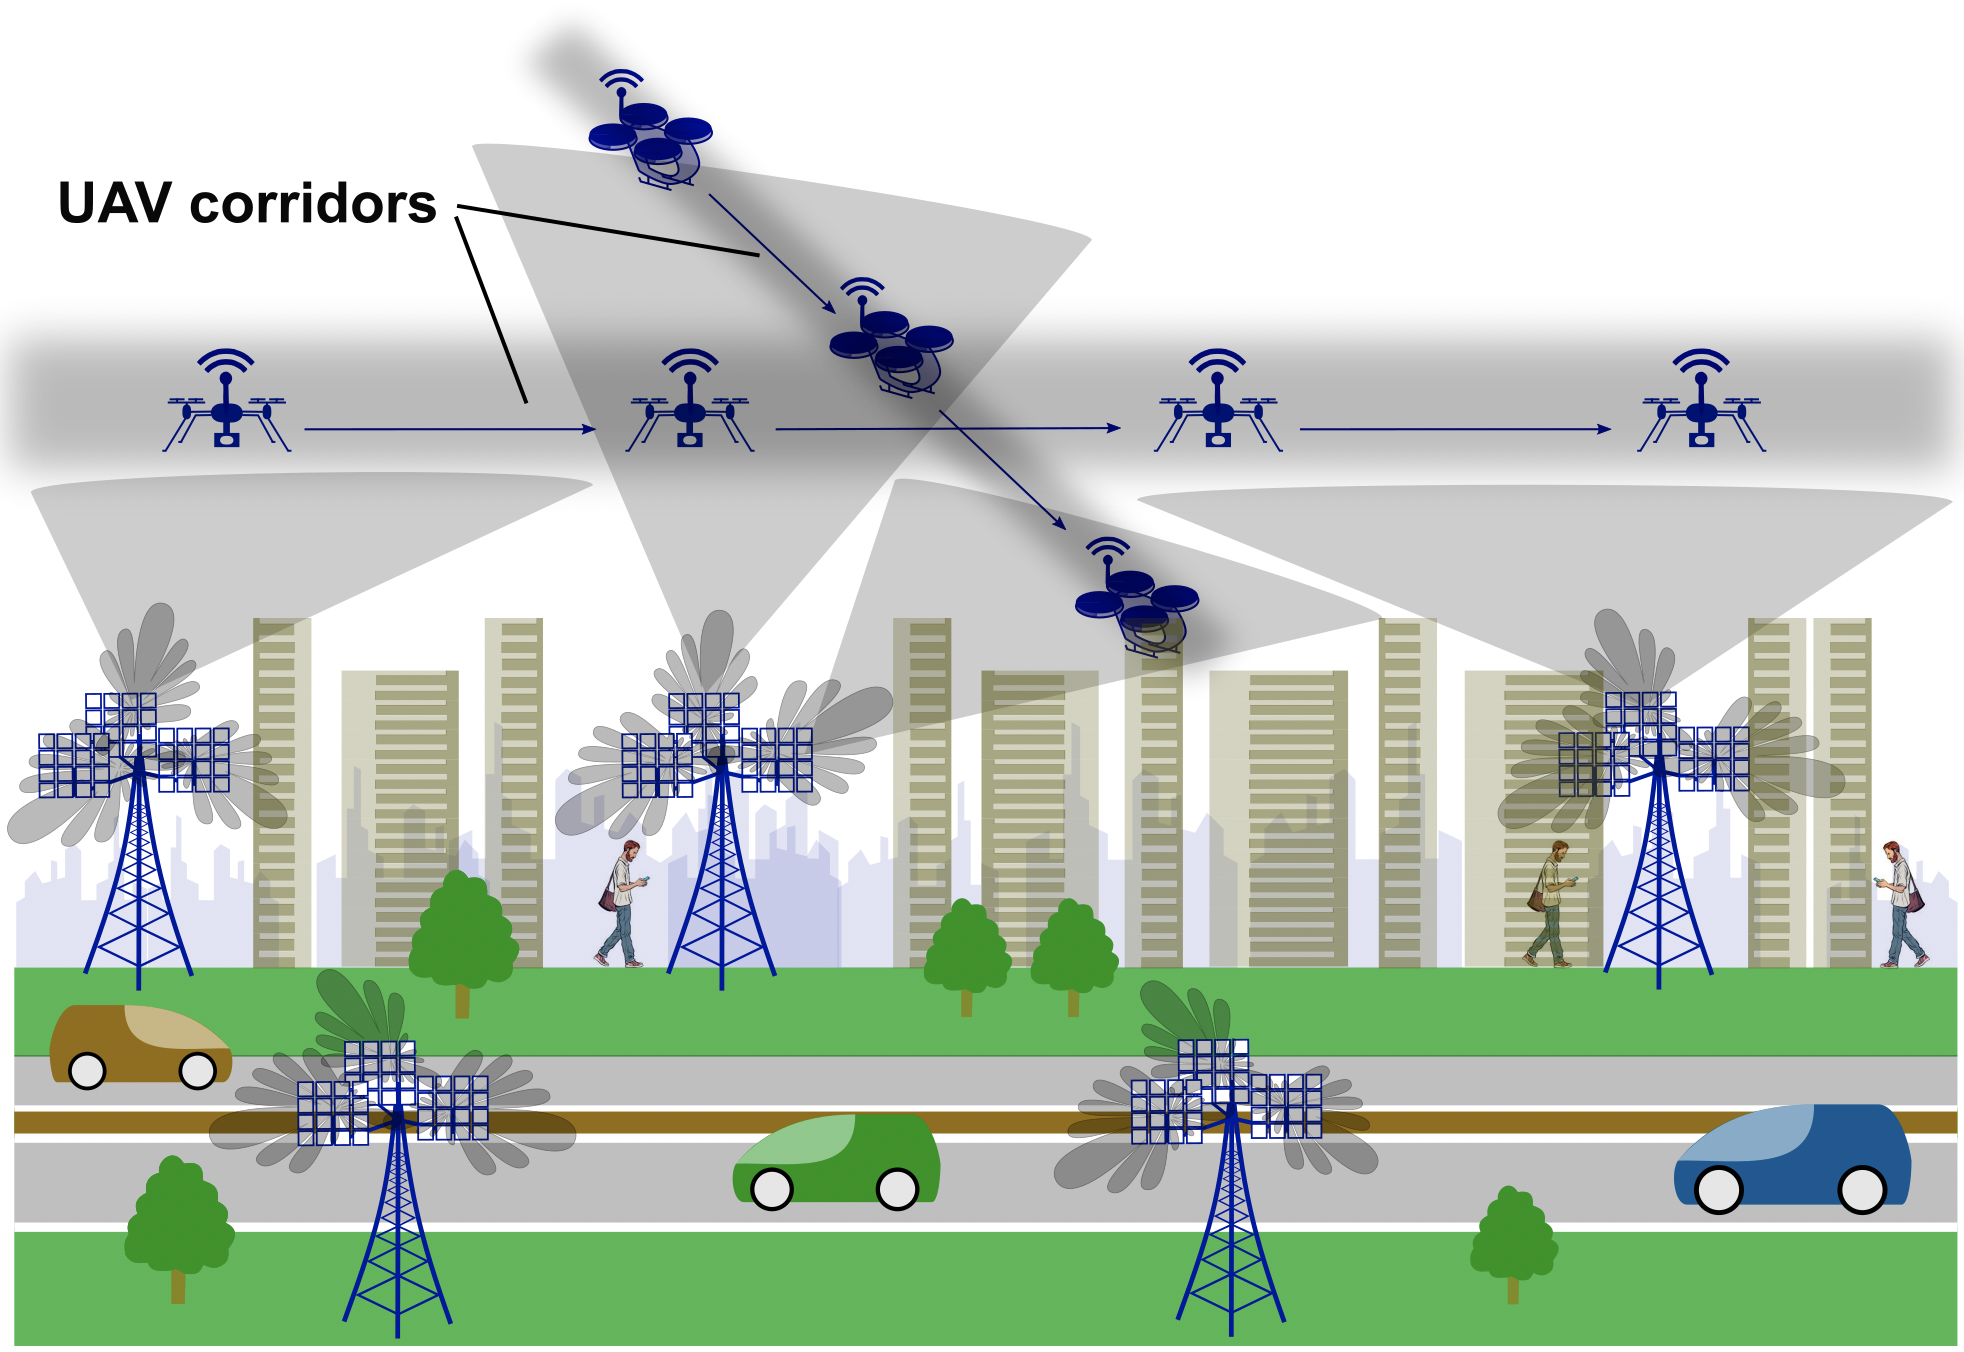
\includegraphics[width=\figwidth]{
Figures/figureCorridors_v03.png}
\caption{Illustration of a cellular network with downtilted and uptilted BSs providing coverage to ground users as well as UAVs flying along corridors (blurred gray).}
\label{fig:illustration}
\end{figure}